\documentclass[spanish]{beamer}

%%% CODIFICACIÓN

\usepackage[utf8]{inputenc}
\usepackage[spanish]{babel}
\usepackage{graphics,tikz}

%%% FUENTES

\usepackage[T1]{fontenc}
\usepackage[familydefault,regular]{}
\usepackage{newtxsf} % Fuente de matemáticas

\setbeamertemplate{navigation symbols}{}

%%% COLORES

\definecolor{background}{RGB}{255,255,255}
\definecolor{text}{RGB}{78,78,78}
\definecolor{accent}{RGB}{6, 105, 125}

\setbeamerfont{framesubtitle}{size=\normalfont\tiny}
\setbeamercolor{framesubtitle}{fg=white}


%%% AJUSTES DE BEAMER

% ¿Negrita en el título de diapositiva o no?
%\setbeamertemplate{frametitle}{\color{accent}\vspace*{1cm}\bfseries\insertframetitle\par\vskip-6pt}

\setbeamertemplate{frametitle}{\color{accent}\vspace*{1cm}\insertframetitle\par\vskip-6pt}

\setbeamertemplate{itemize items}[circle] % Viñetas de itemize

%%% CONFIGURACIÓN DE COLORES DE BEAMER

\setbeamercolor{background canvas}{bg=background}
\setbeamercolor{normal text}{fg=text}
\setbeamercolor{alerted text}{fg=accent}
\setbeamercolor{block title}{fg=accent}
\setbeamercolor{alerted text}{fg=accent}
\setbeamercolor{itemize item}{fg=accent}
\setbeamercolor{enumerate item}{fg=accent}
\setbeamercolor*{title}{fg=accent}
\setbeamercolor{qed symbol}{fg=accent}
\usebeamercolor[fg]{normal text}

%%% INFORMACIÓN DEL DOCUMENTO

\title{Metologías de Desarrollo Ágil : práctica 4}
\subtitle{Tablero trello y kanban de la iteración 1}
\author{Miguel Albertí Pons\\ Sofía Almeida Bruno\\ Pedro Manuel Flores Crespo\\ María Victoria Granados Pozo\\ Lidia Martín Chica\vspace{1em}Grupo 2}


\begin{document}

\maketitle

\begin{frame}
\centering
\begin{center}
		
\includegraphics[scale=0.4]{../../Imagenes/Logo}
	\end{center}
\end{frame}

\begin{frame}
\centering
	\begin{center}
		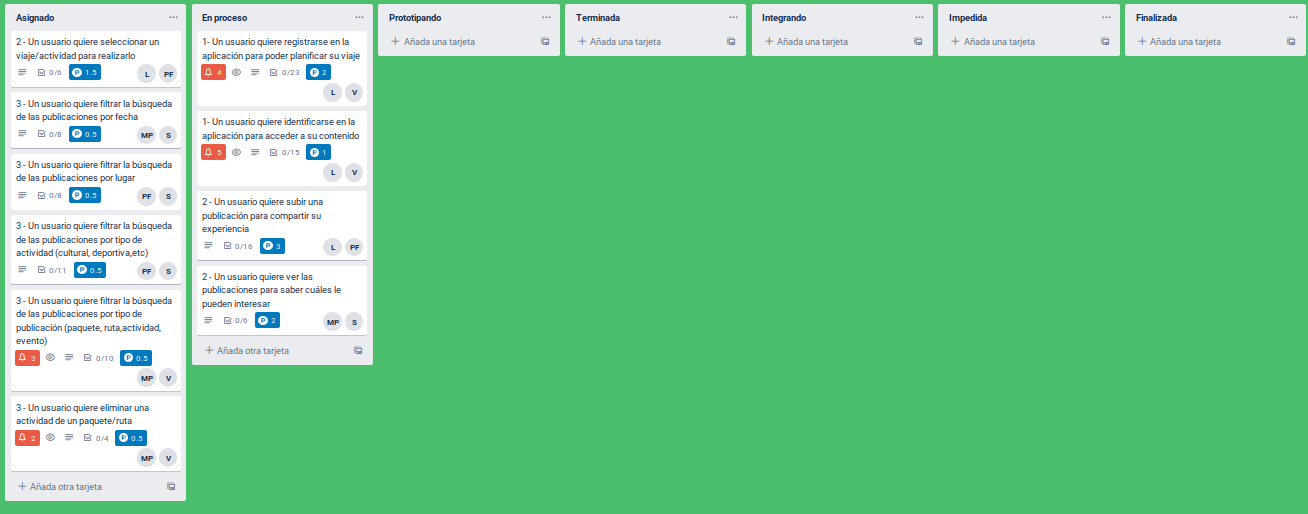
\includegraphics[scale=0.25]{trello1_1}
	\end{center}
\end{frame}


\begin{frame}
	\begin{center}
		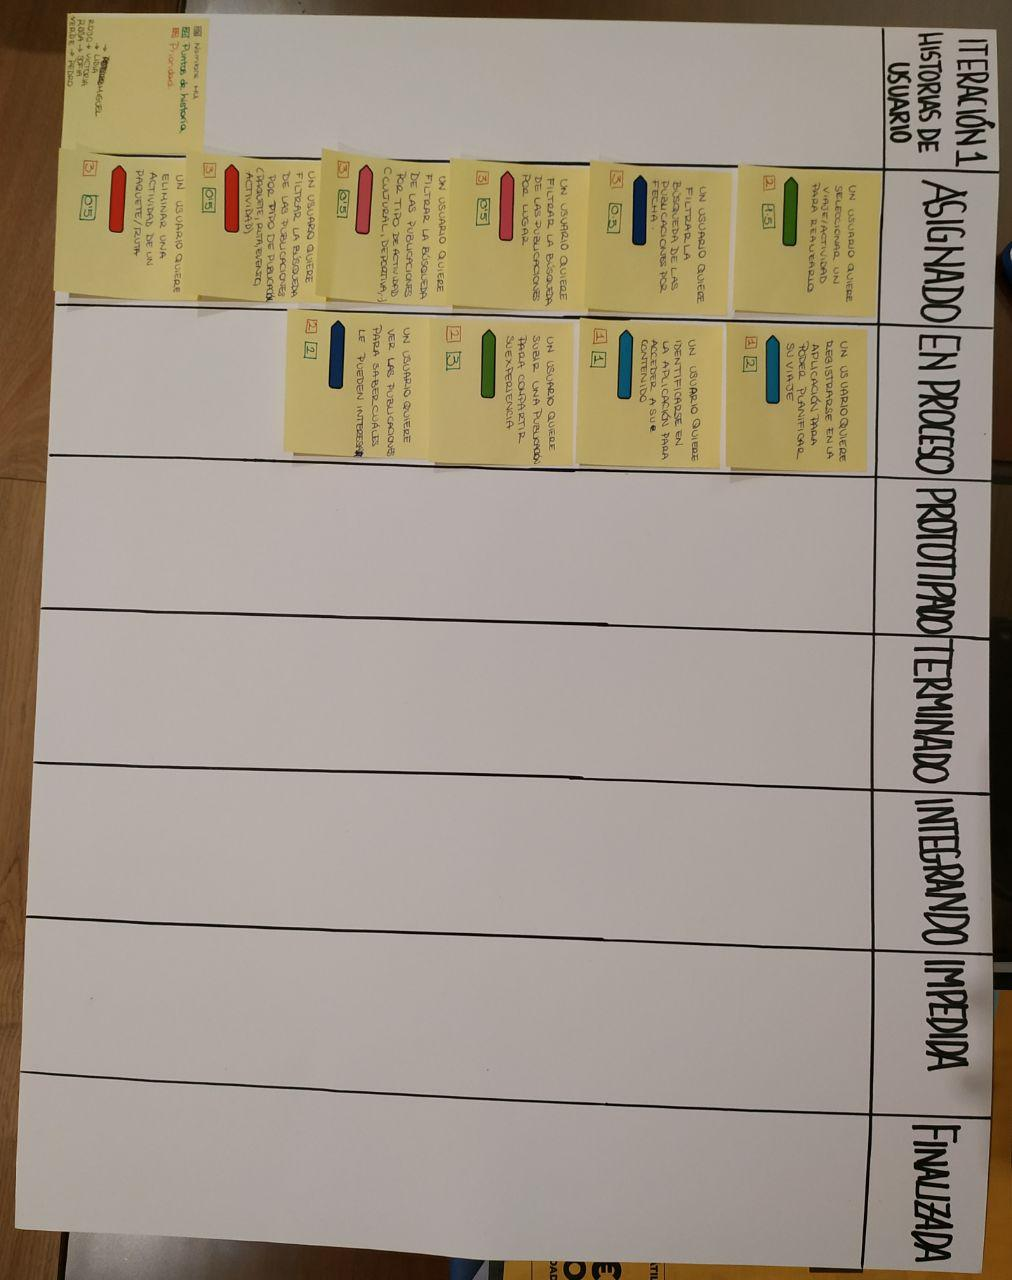
\includegraphics[angle=90, scale=0.32]{papel1_1}
	\end{center}
\end{frame}

\begin{frame}
	\begin{center}
		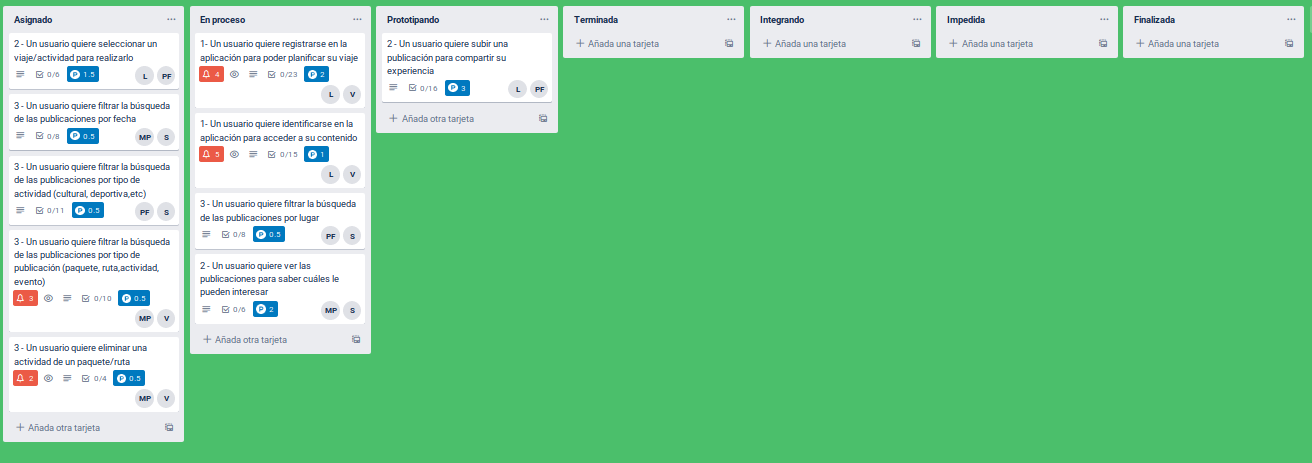
\includegraphics[scale=0.25]{trello1_2}
	\end{center}
\end{frame}

\begin{frame}
	\begin{center}
		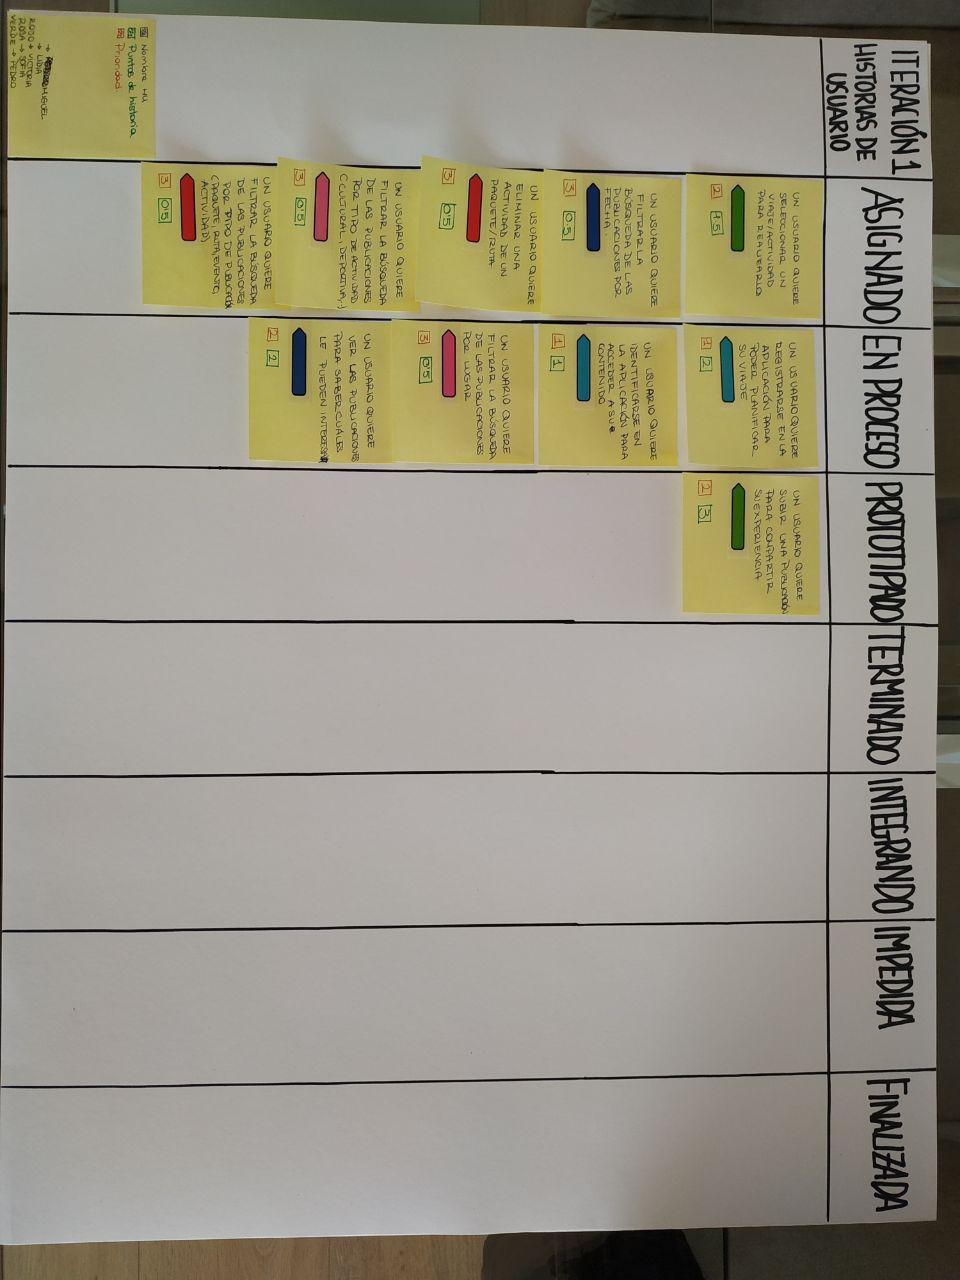
\includegraphics[angle=90, scale=0.33]{papel1_2}
	\end{center}
\end{frame}

\begin{frame}
	\begin{center}
		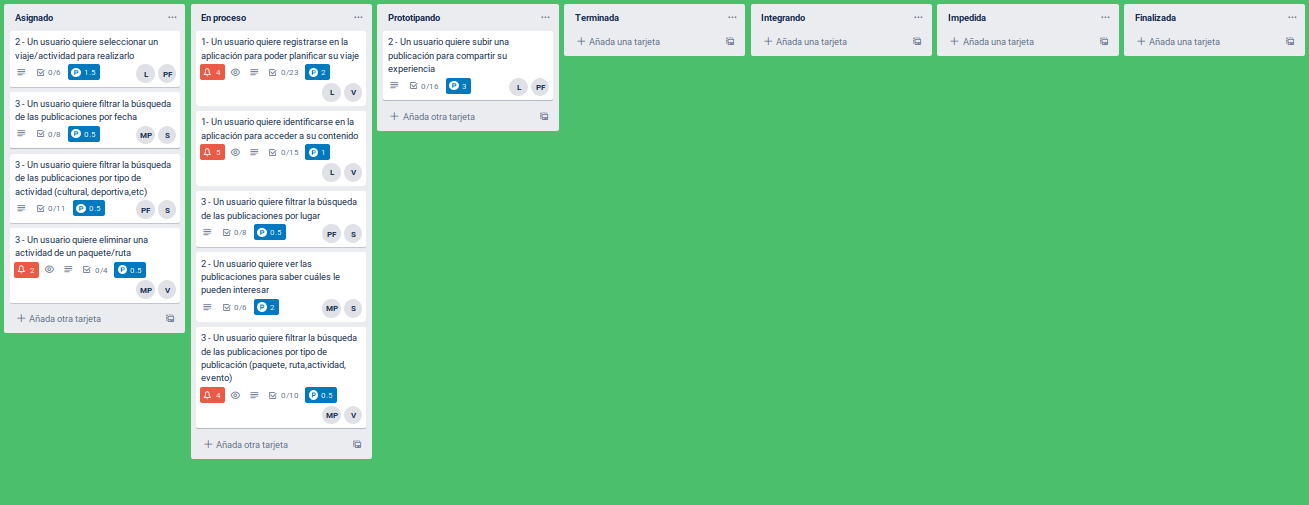
\includegraphics[scale=0.24]{trello1_3}
	\end{center}
\end{frame}

\begin{frame}
	\begin{center}
		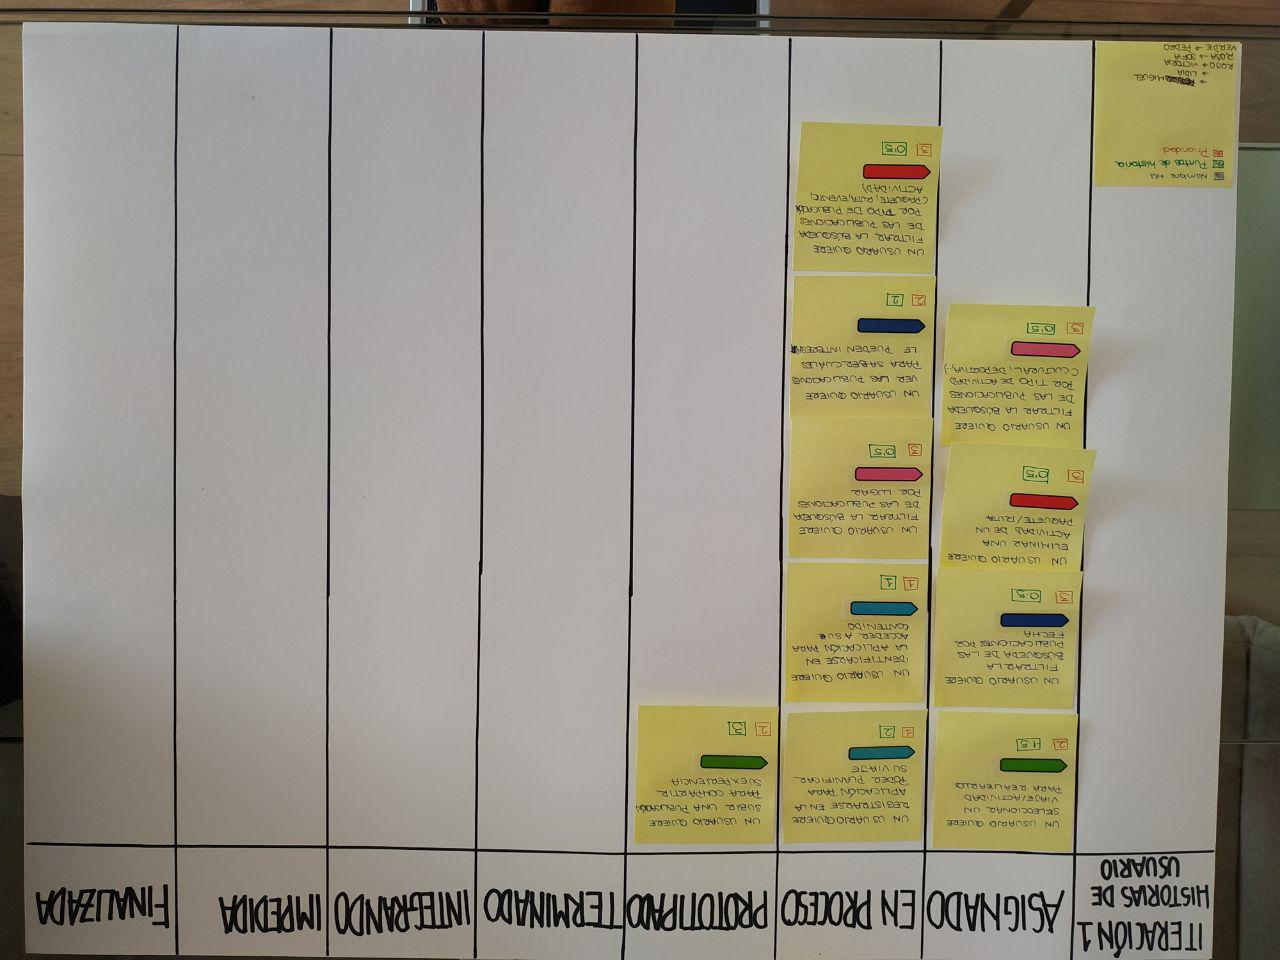
\includegraphics[angle=180, scale=0.32]{papel1_3}
	\end{center}
\end{frame}

\begin{frame}
	\begin{center}
		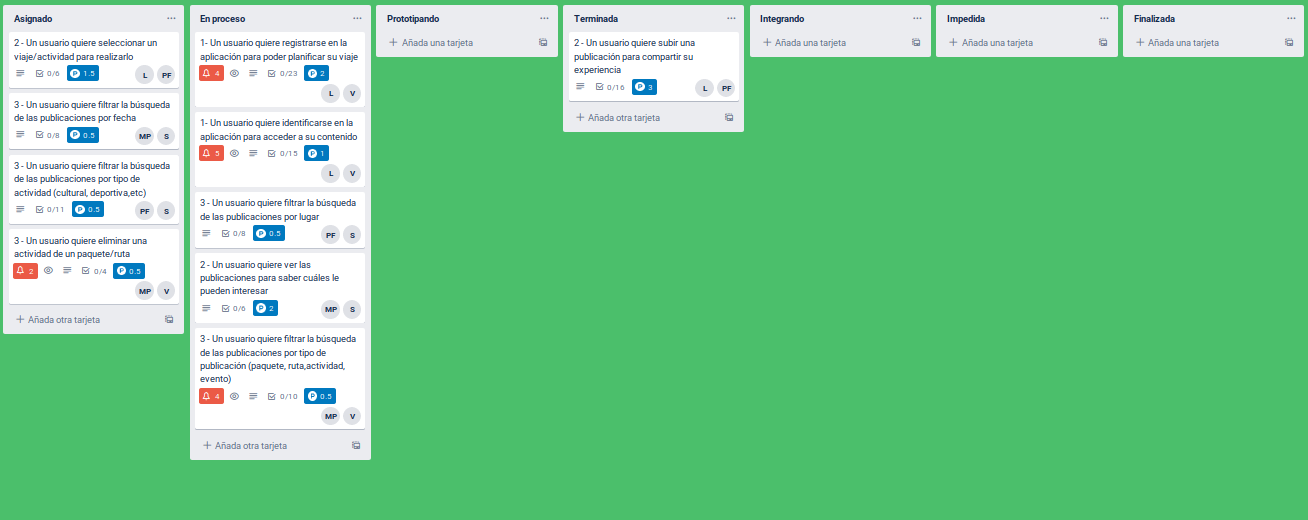
\includegraphics[scale=0.24]{trello1_4}
	\end{center}
\end{frame}

\begin{frame}
	\begin{center}
		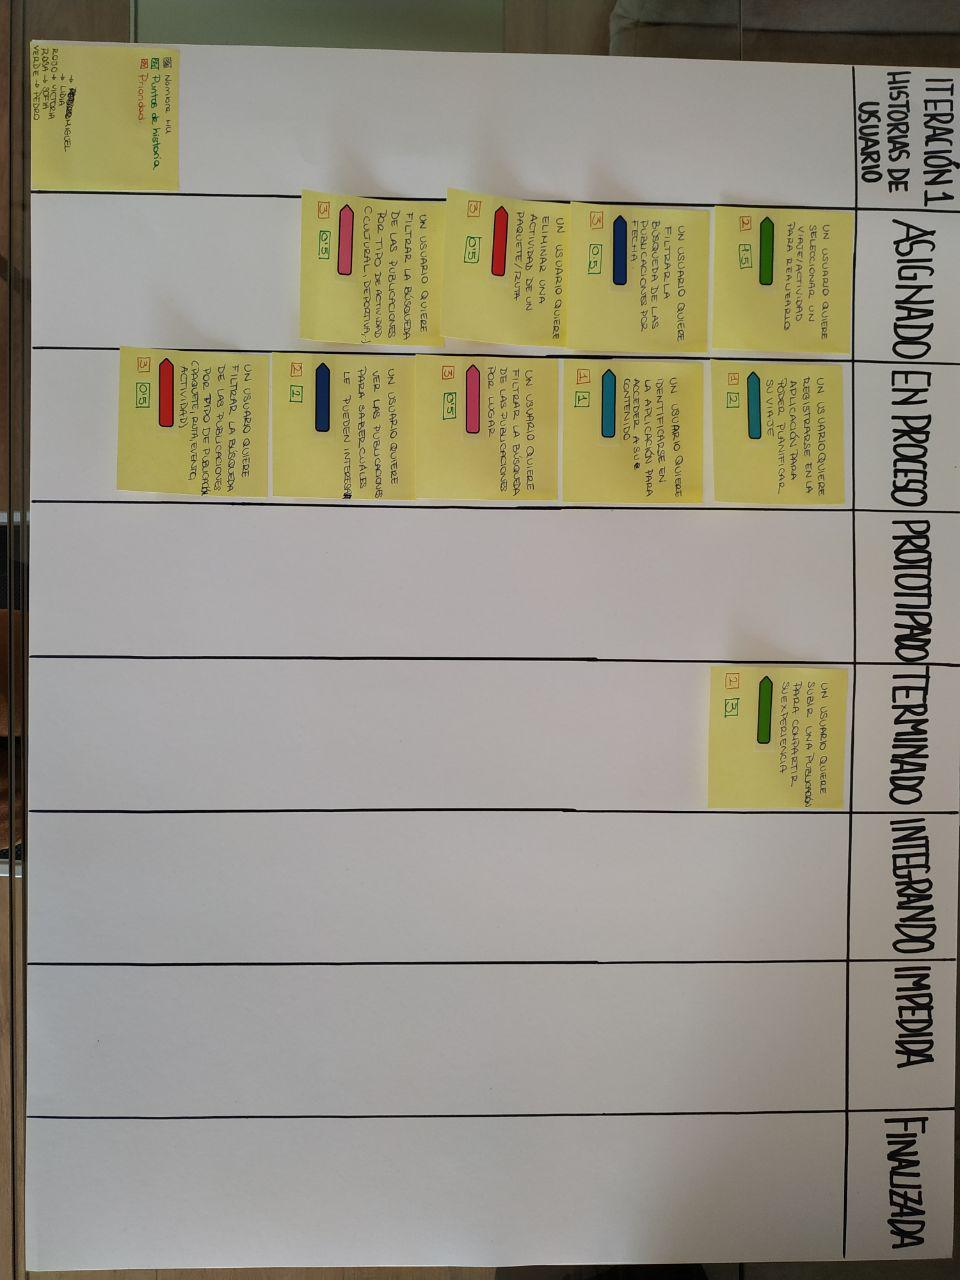
\includegraphics[angle=90, scale=0.34]{papel1_4}
	\end{center}
\end{frame}

\begin{frame}
	\begin{center}
		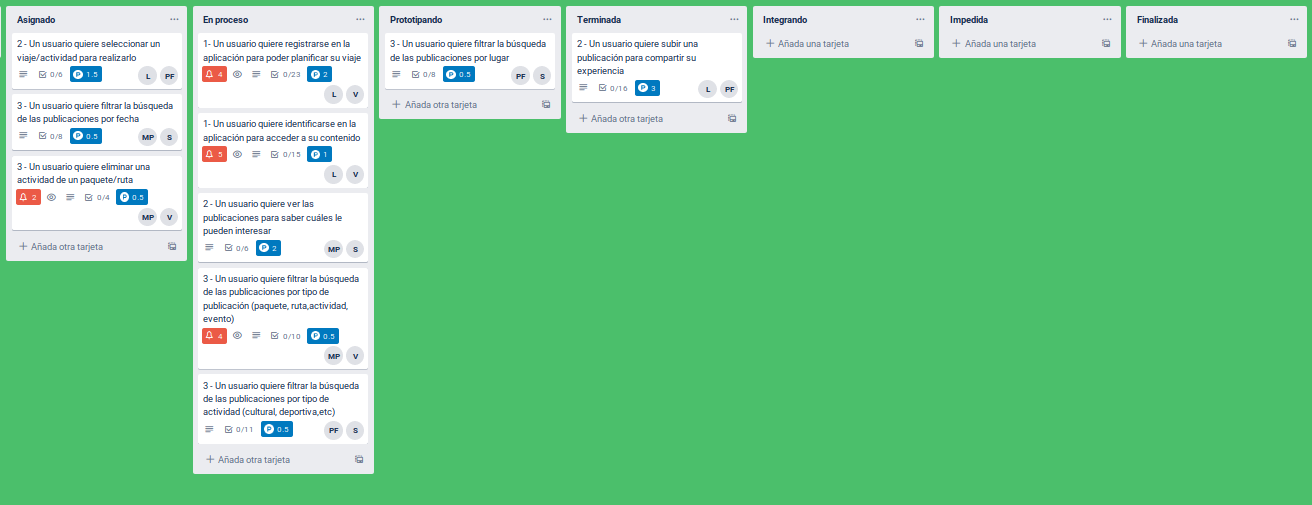
\includegraphics[scale=0.24]{trello1_5}
	\end{center}
\end{frame}

\begin{frame}
	\begin{center}
		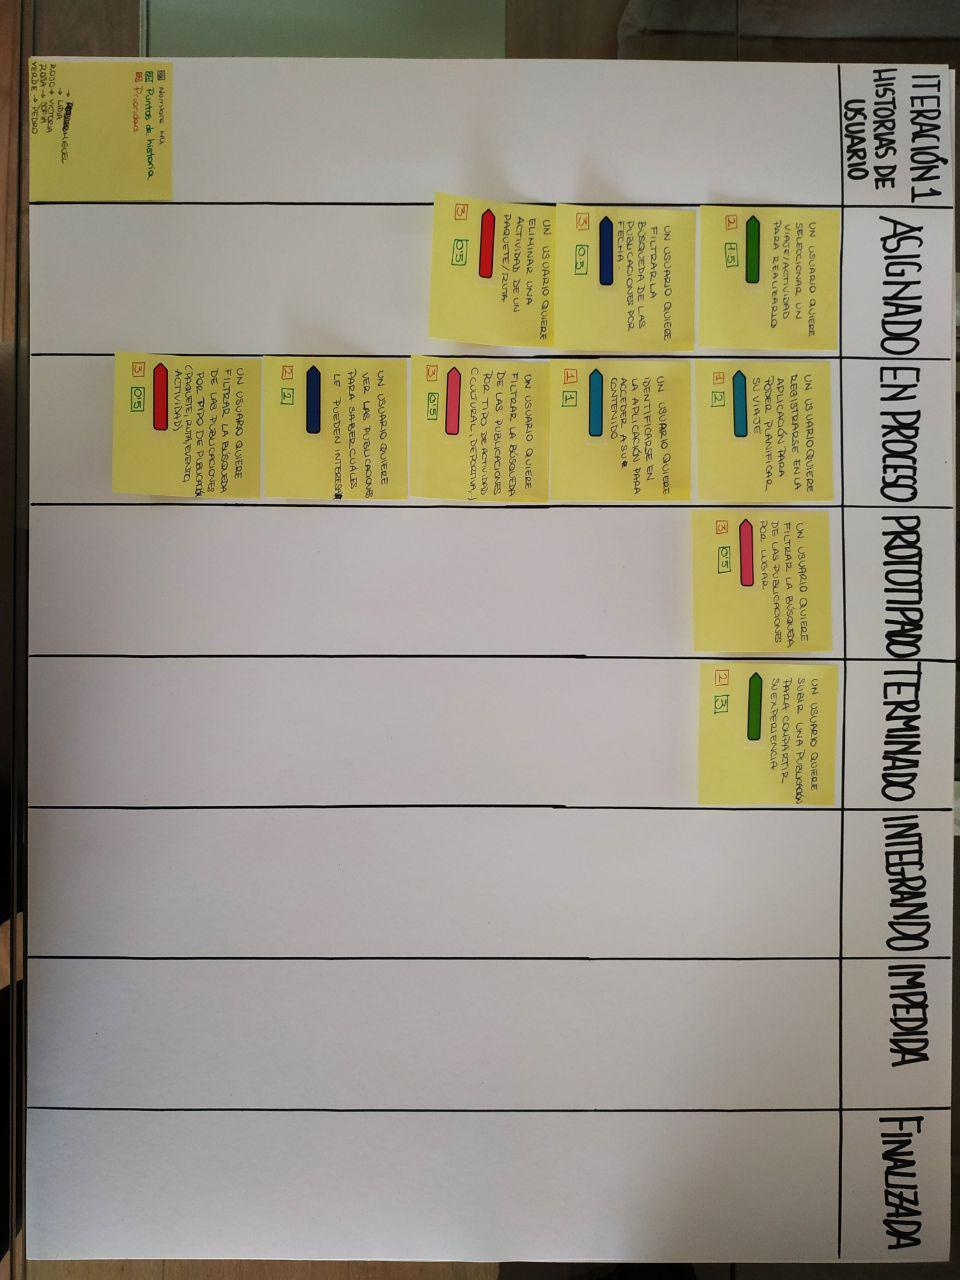
\includegraphics[angle=90, scale=0.335]{papel1_5}
	\end{center}
\end{frame}

\begin{frame}
	\begin{center}
		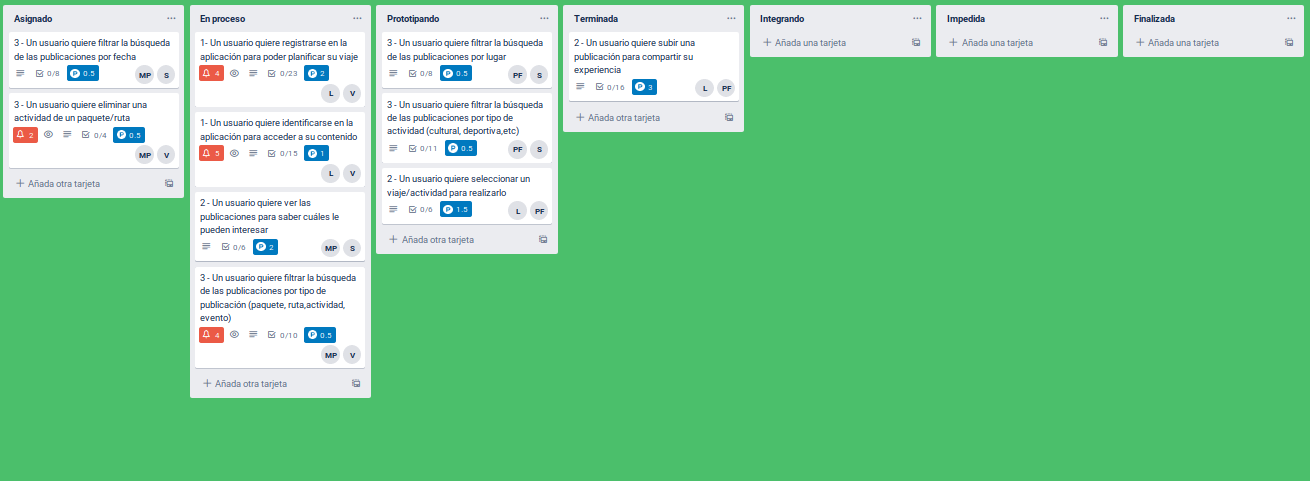
\includegraphics[scale=0.25]{trello1_6}
	\end{center}
\end{frame}

\begin{frame}
	\begin{center}
		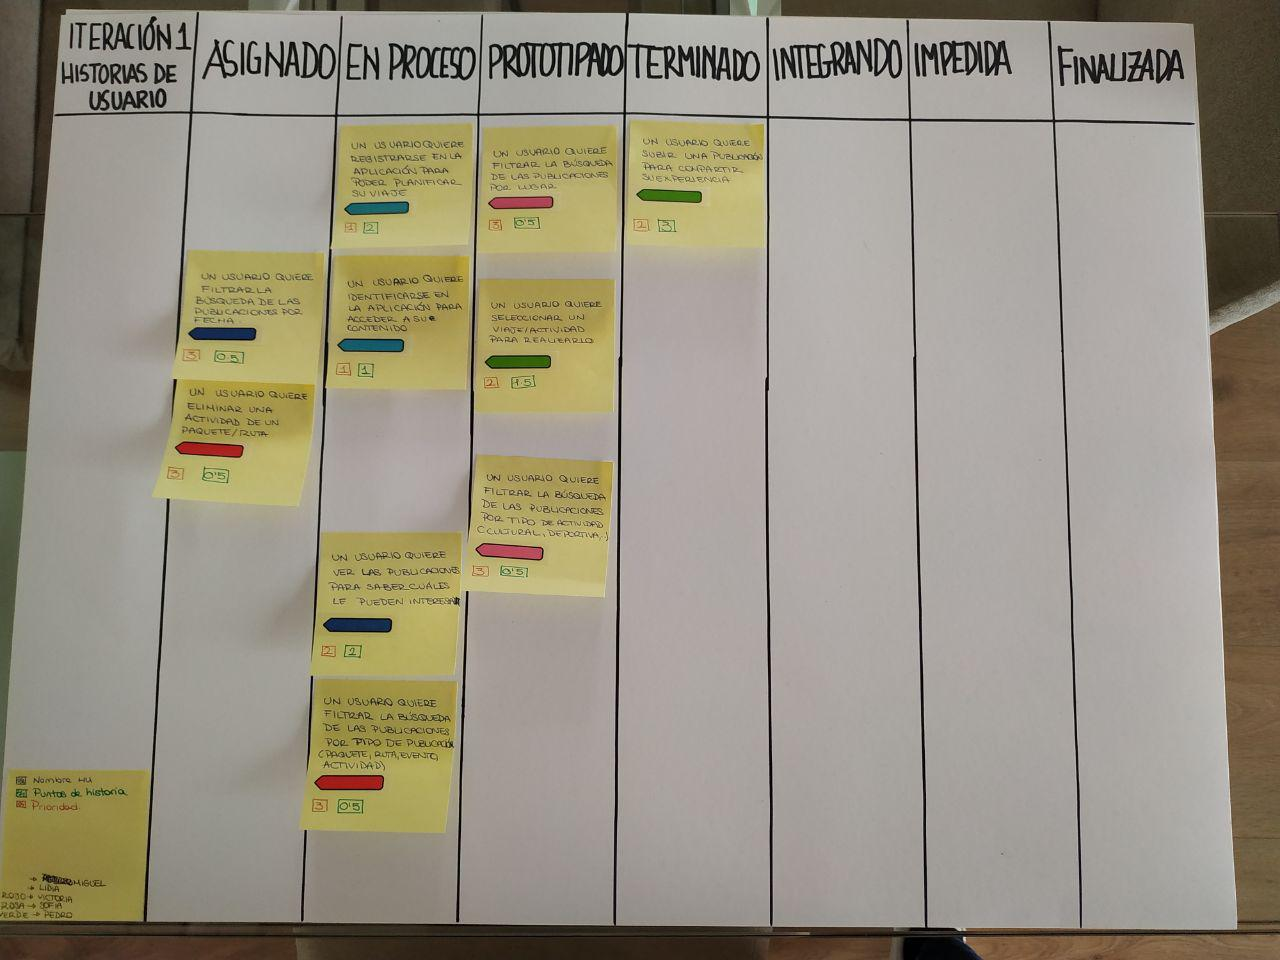
\includegraphics[angle=0, scale=0.34]{papel1_6}
	\end{center}
\end{frame}

\begin{frame}
	\begin{center}
		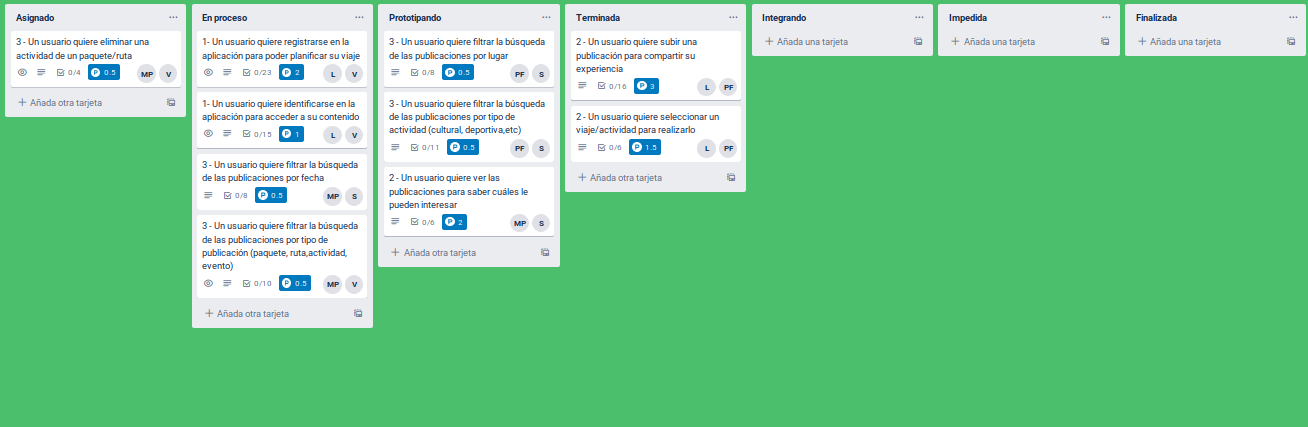
\includegraphics[scale=0.25]{trello1_7}
	\end{center}
\end{frame}

\begin{frame}
	\begin{center}
		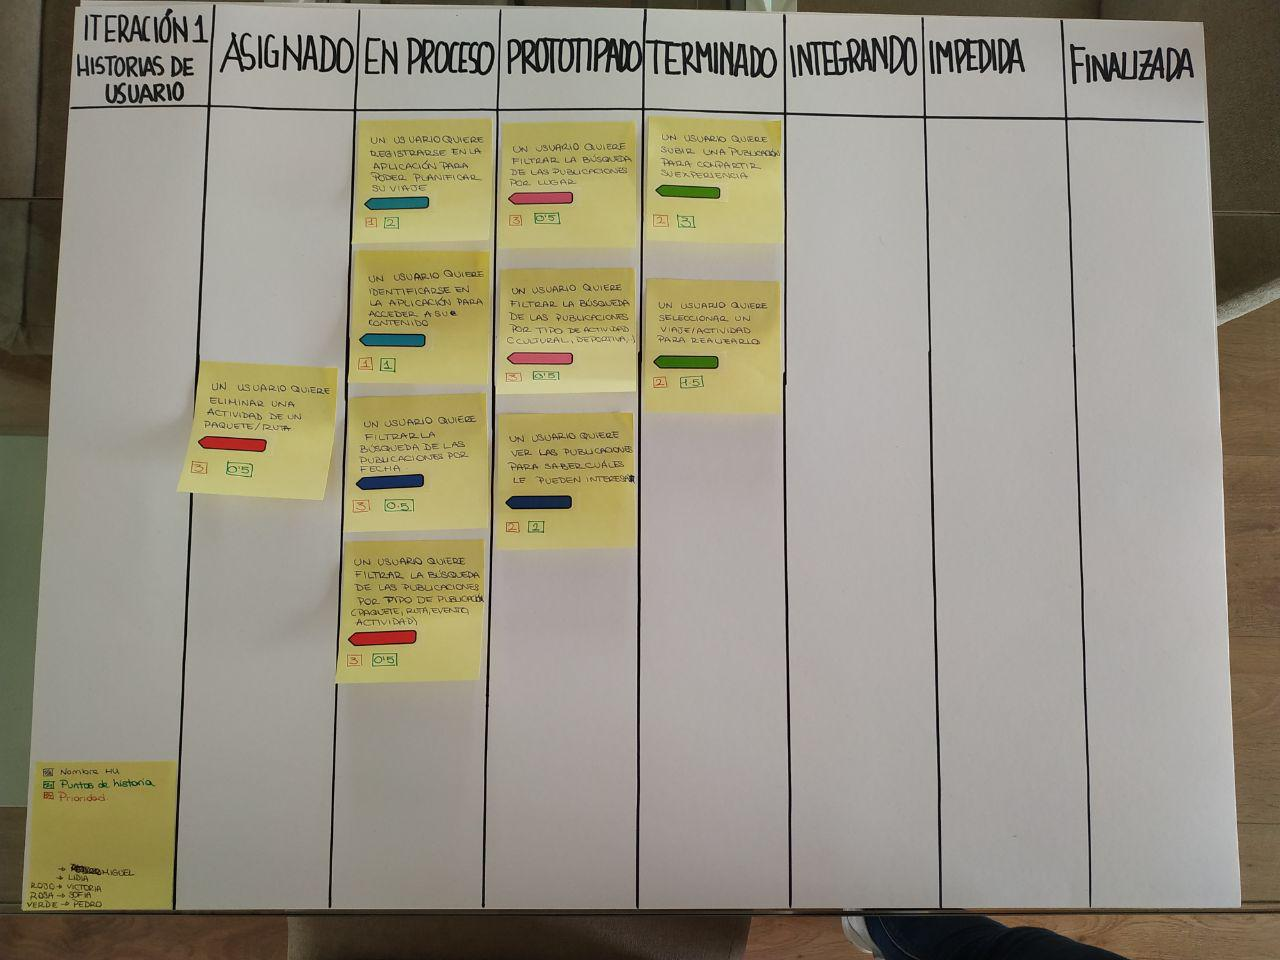
\includegraphics[scale=0.34]{papel1_7}
	\end{center}
\end{frame}

\begin{frame}
	\begin{center}
		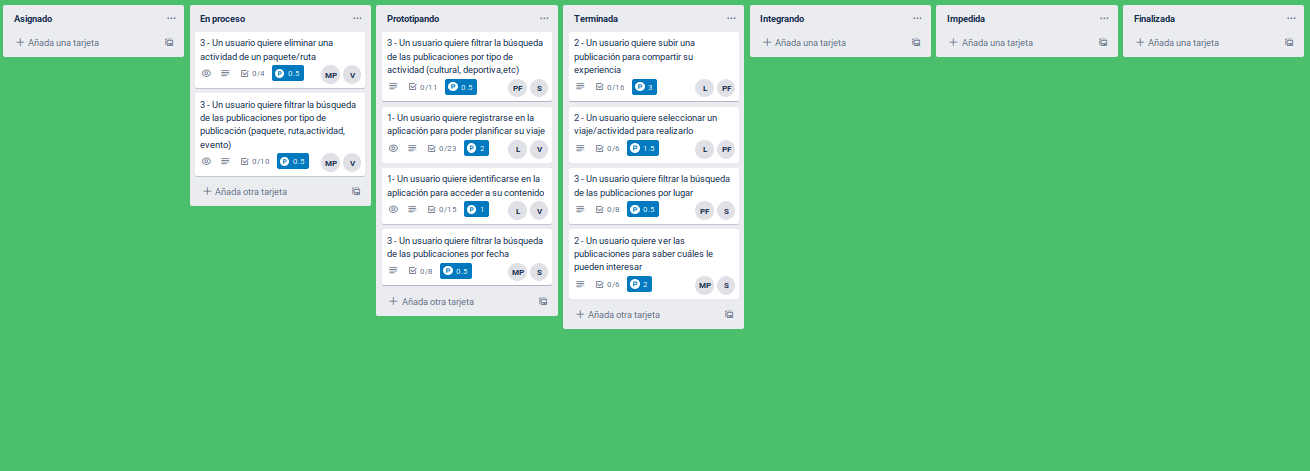
\includegraphics[scale=0.25]{trello1_8}
	\end{center}
\end{frame}

\begin{frame}
	\begin{center}
		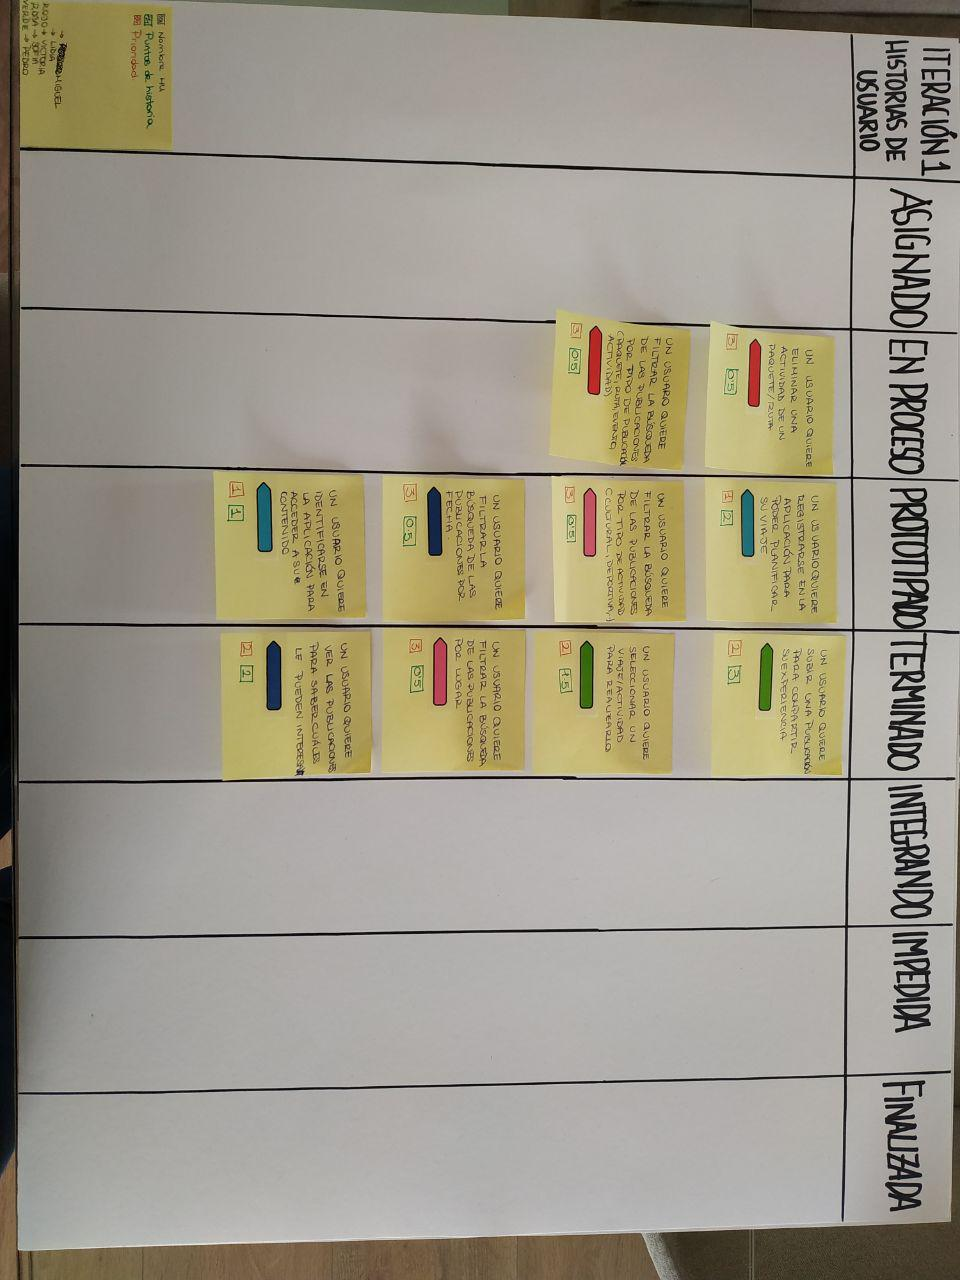
\includegraphics[angle=90, scale=0.34]{papel1_8}
	\end{center}
\end{frame}

\begin{frame}
	\begin{center}
		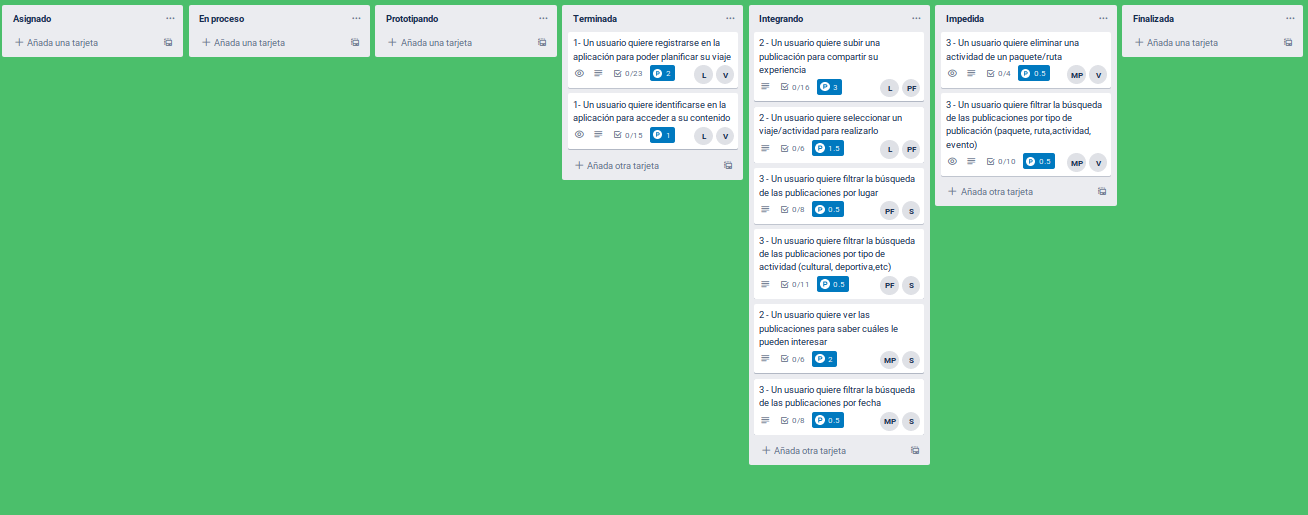
\includegraphics[scale=0.25]{trello1_9}
	\end{center}
\end{frame}

\begin{frame}
	\begin{center}
		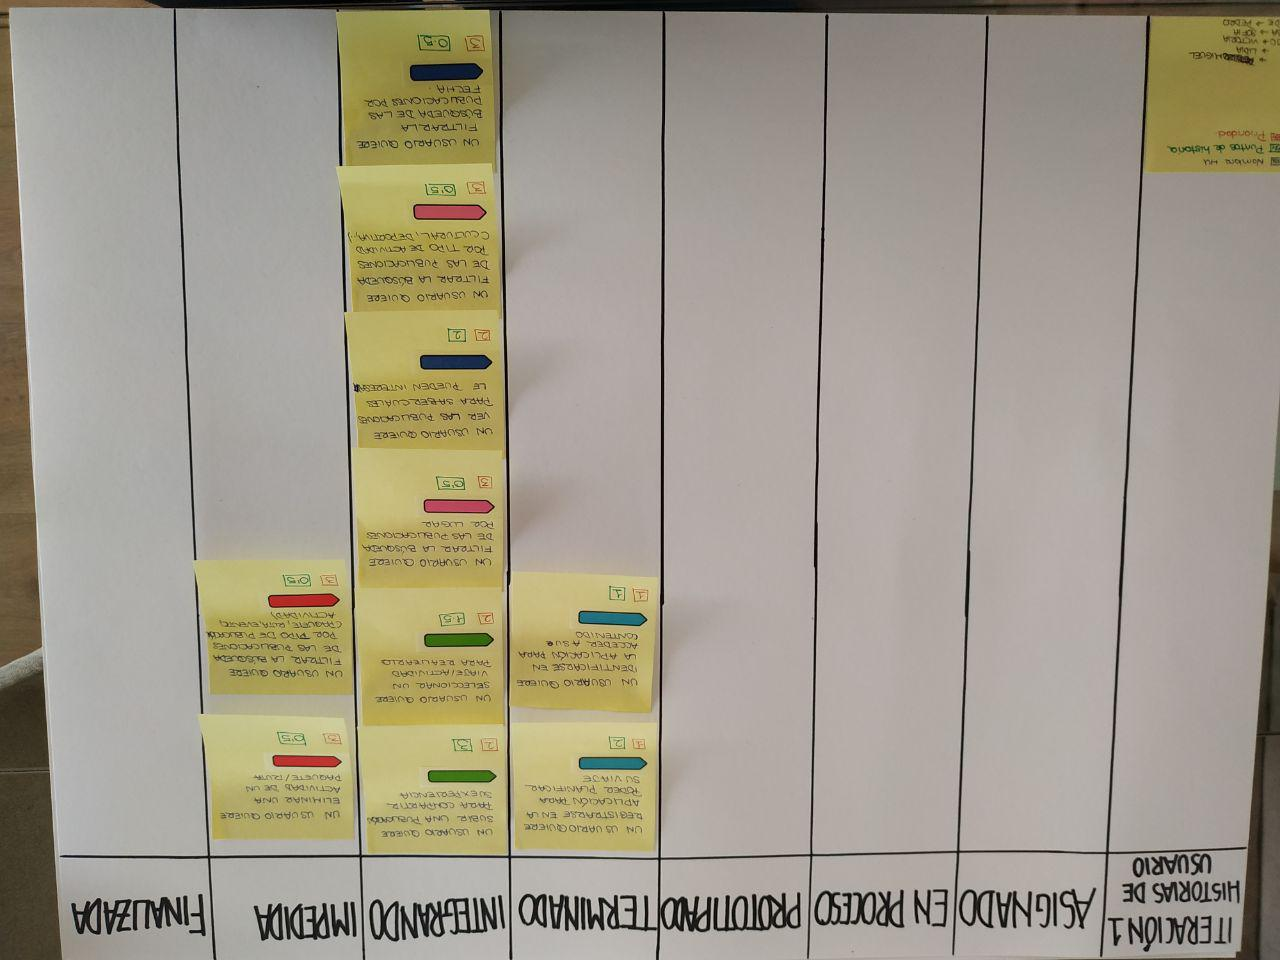
\includegraphics[angle=180, scale=0.33]{papel1_9}
	\end{center}
\end{frame}



\end{document}

